
\subsection{Relaxing anticipation assumption}%
\label{sub:relaxing_anticipation_assumption}

\begin{itemize}
    \item In our setting where users self-select into signing app to the app,
        it is possible that our results are influenced by anticipation effects.

    \item In particular, it is possible that users started to cut back on
        discretionary spend a few months before signing up to the app. In this
    case, our estimates in Figure~\ref{fig:main_results} would underestimate

    \item Three reasonable scenarios: users just deciding to sign up for
        reasons unrelated to trajectory of dspend, decidign to cut back a few
        months earlier and wanting additional help, looking for tool to help
        them curb increase in dspend.

    \item Raw data is consistent with third story.

    \item Anticipation doesn't seem to be an issue.

    \item Raw data also explains why increase of anticipation window reduces
        effect: spend increased month by month. Anticipation moves reference
        period back. The further back reference periods, the closer dspend is
        to post signup.


    \item As \citet{callaway2021difference} point out in Remark 1, the parallel
        trend assumption becomes stronger as we increase delta, since parallel
        trends are now required to hold also in periods prior to actual
        treatment.

    \item In our setup, this is not the case, due to self-selection:
        pre-treatment periods differ for treated and untreated units because
        treated units tend to experience higher dspend before signup, which
        might be what causes them to sign up.

\end{itemize}

\begin{figure}[H]
    \centering
    \caption{Anticipation ...}%
    \label{fig:new}
    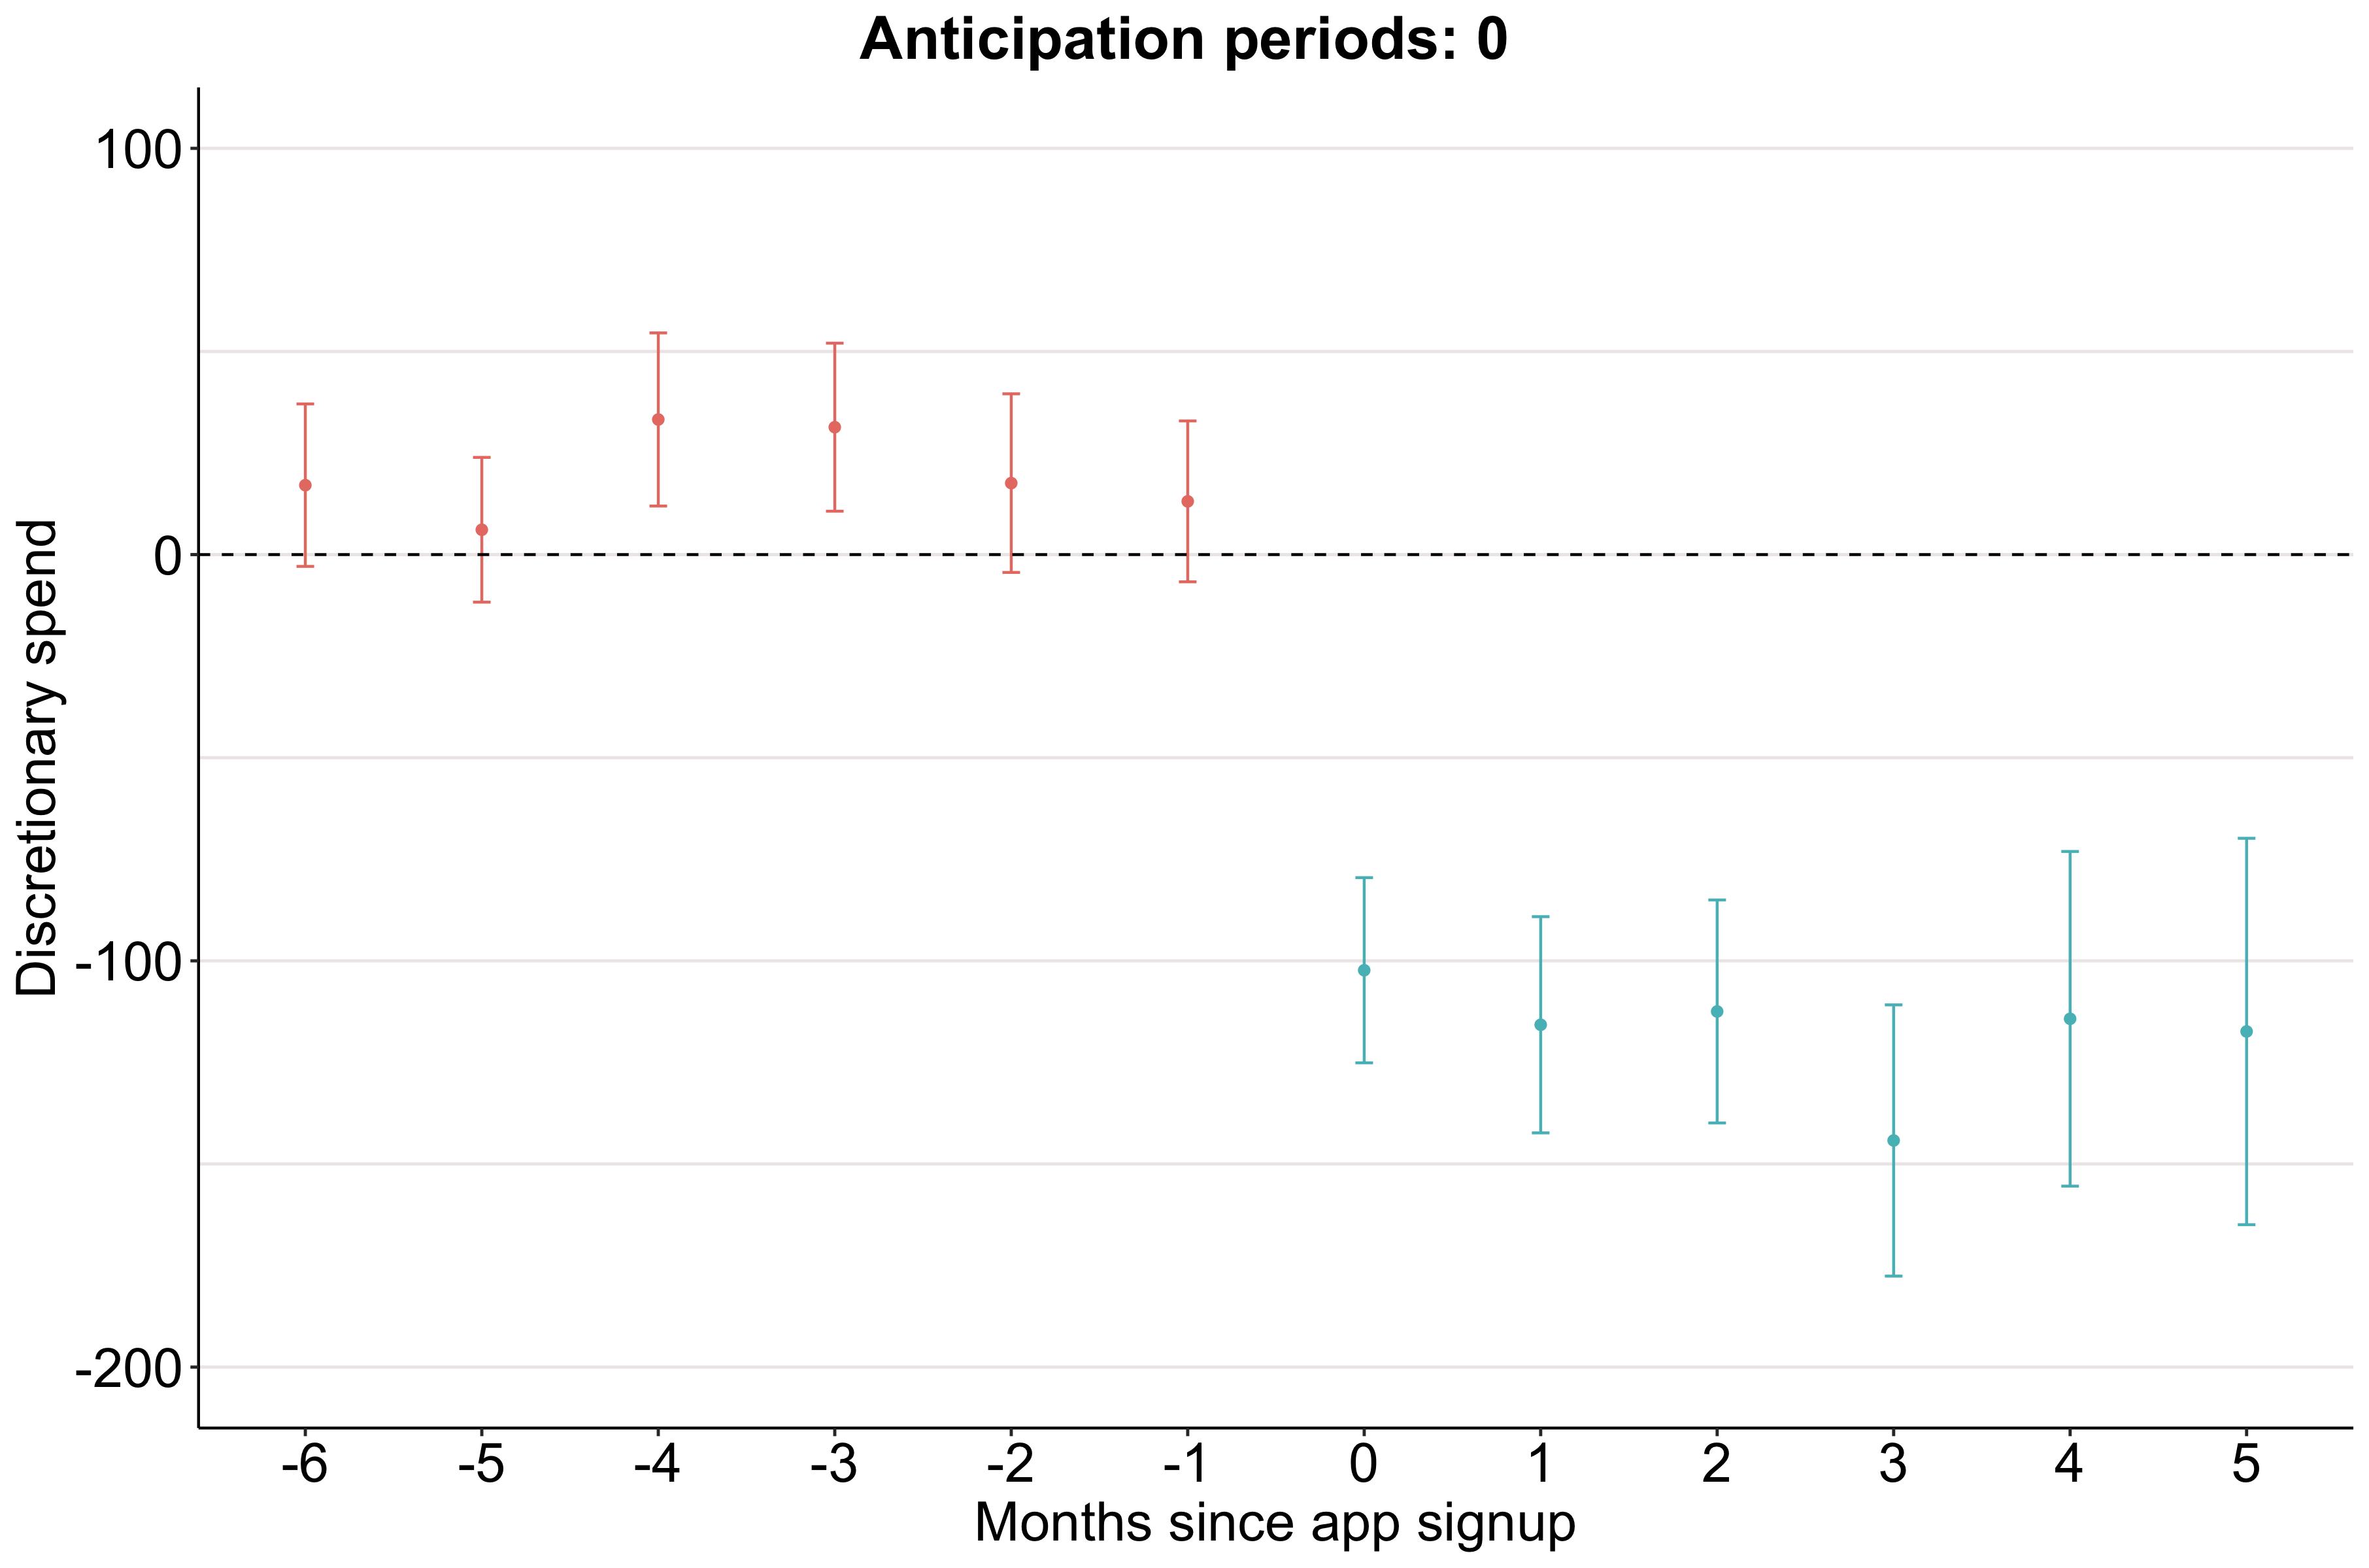
\includegraphics[width=.24\textwidth]{\figdir/dspend_antic0_es.png}
    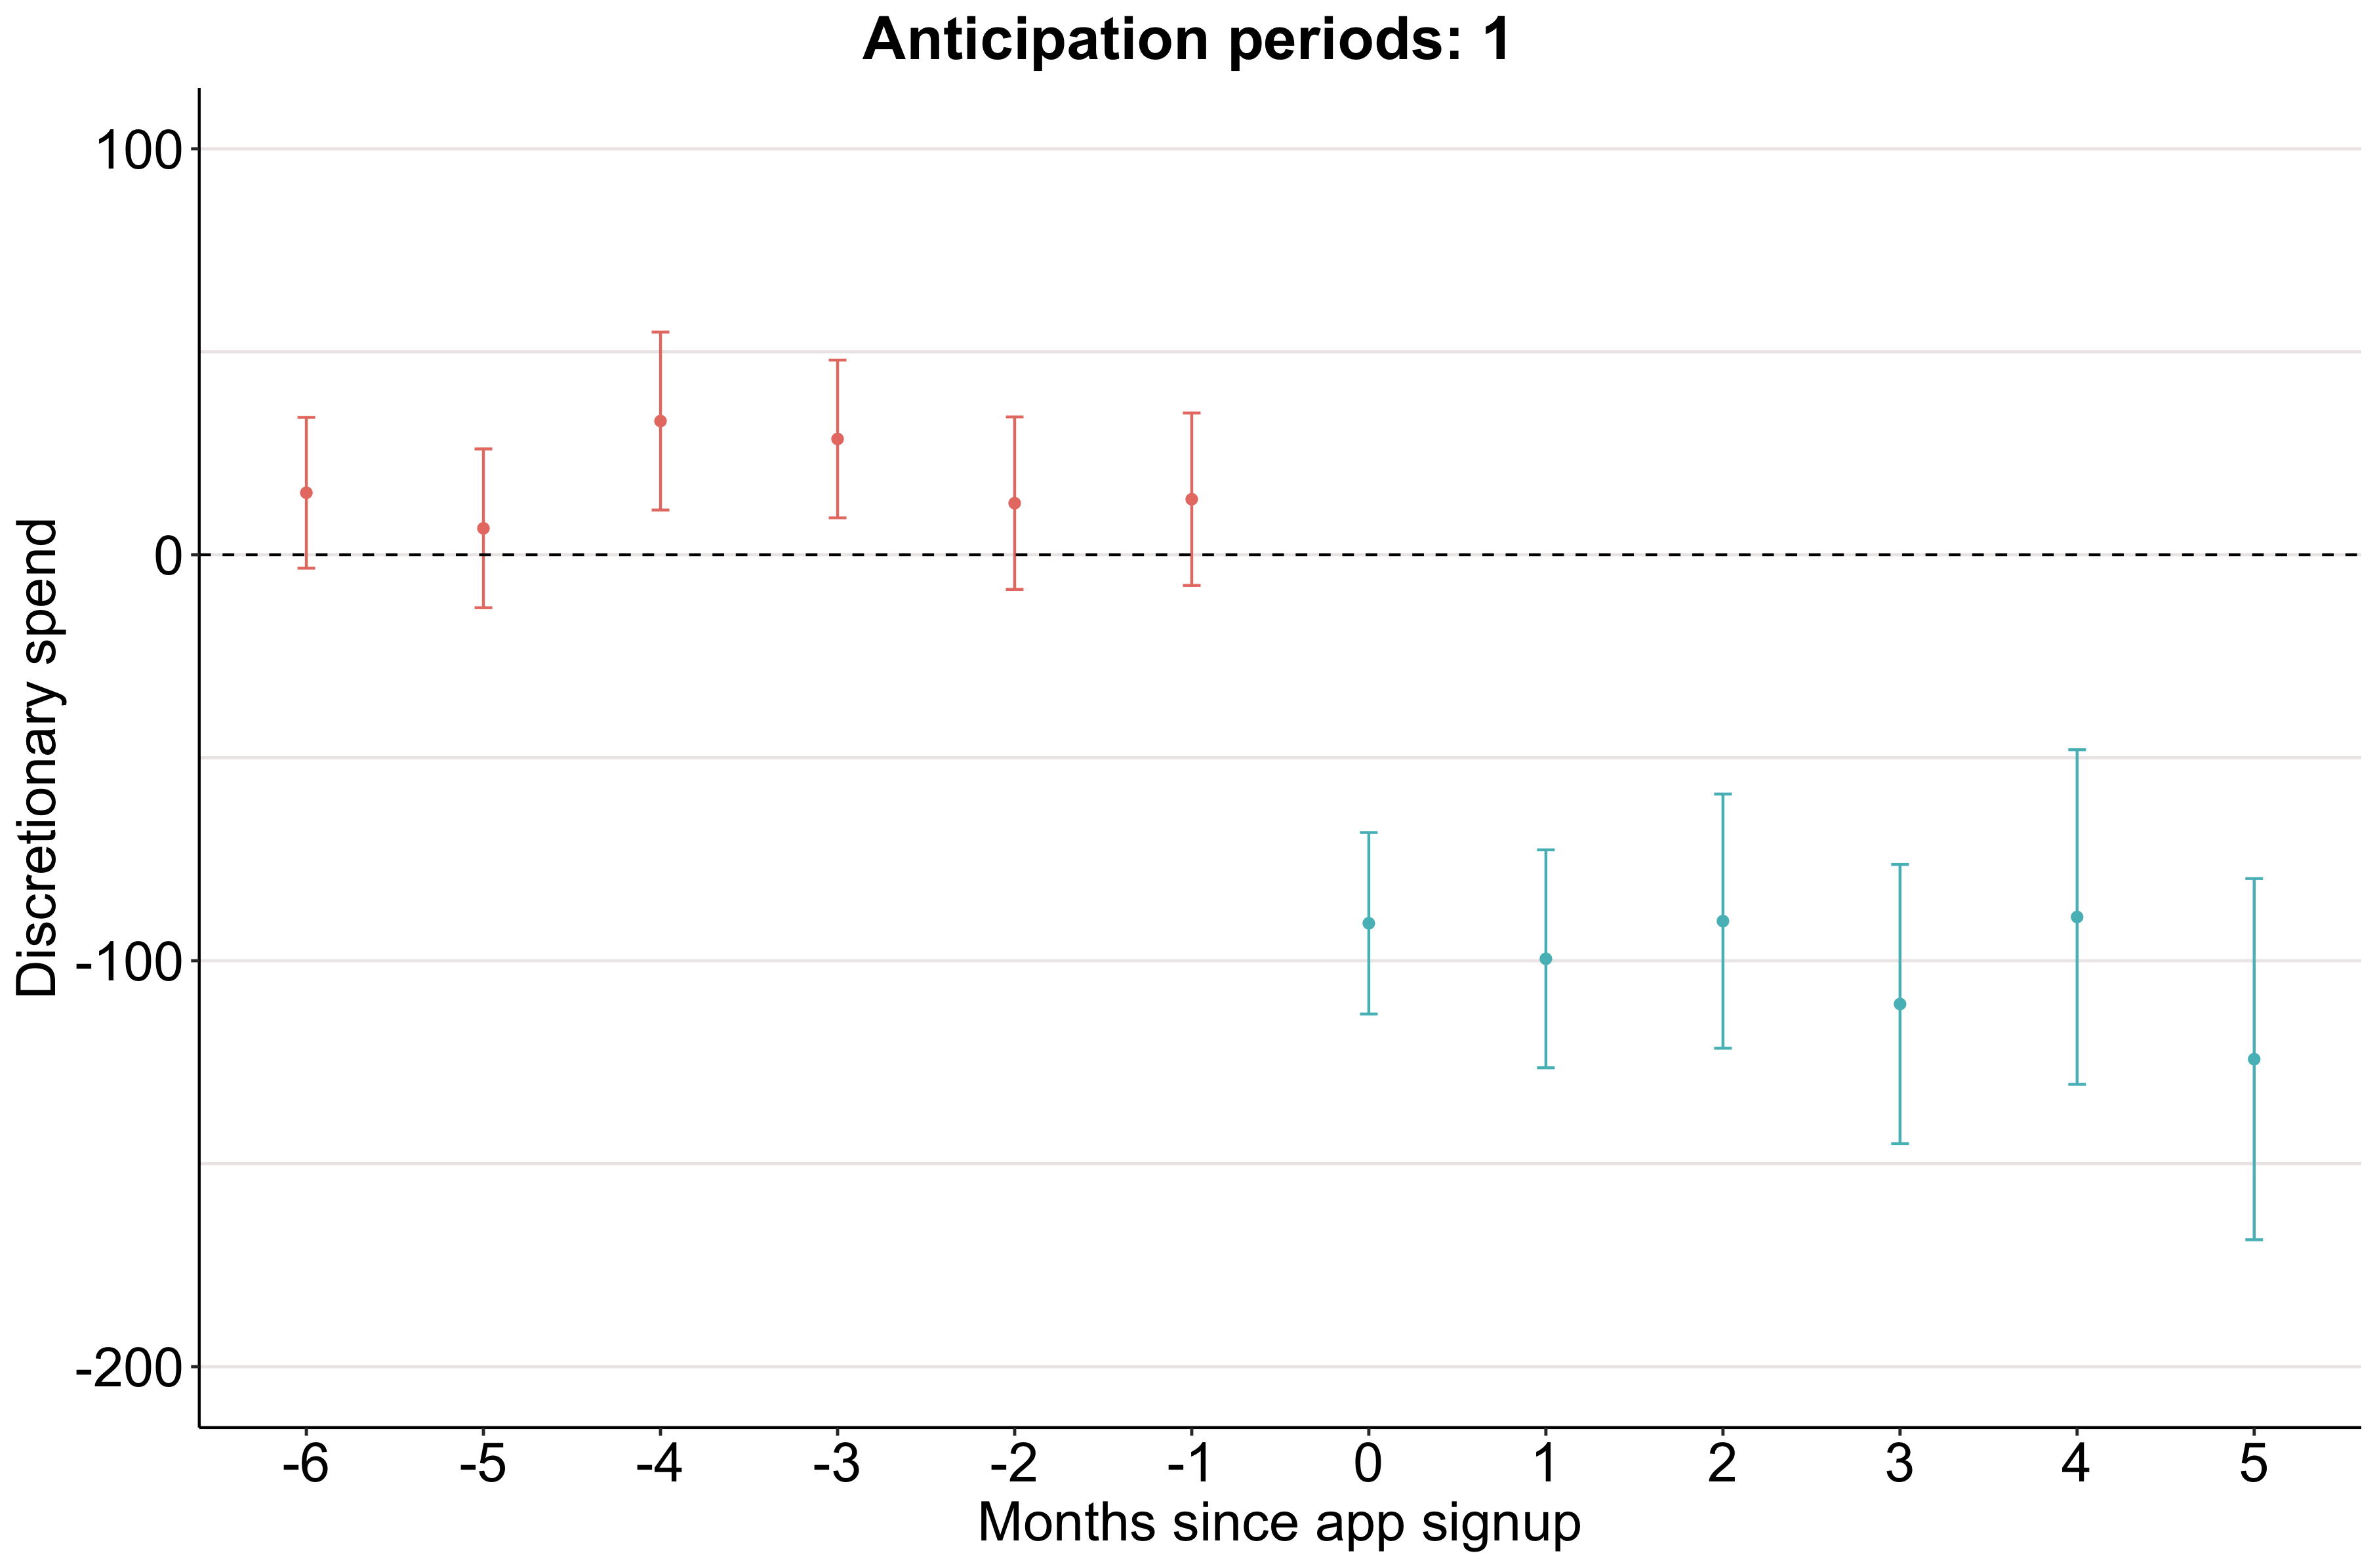
\includegraphics[width=.24\textwidth]{\figdir/dspend_antic1_es.png}
    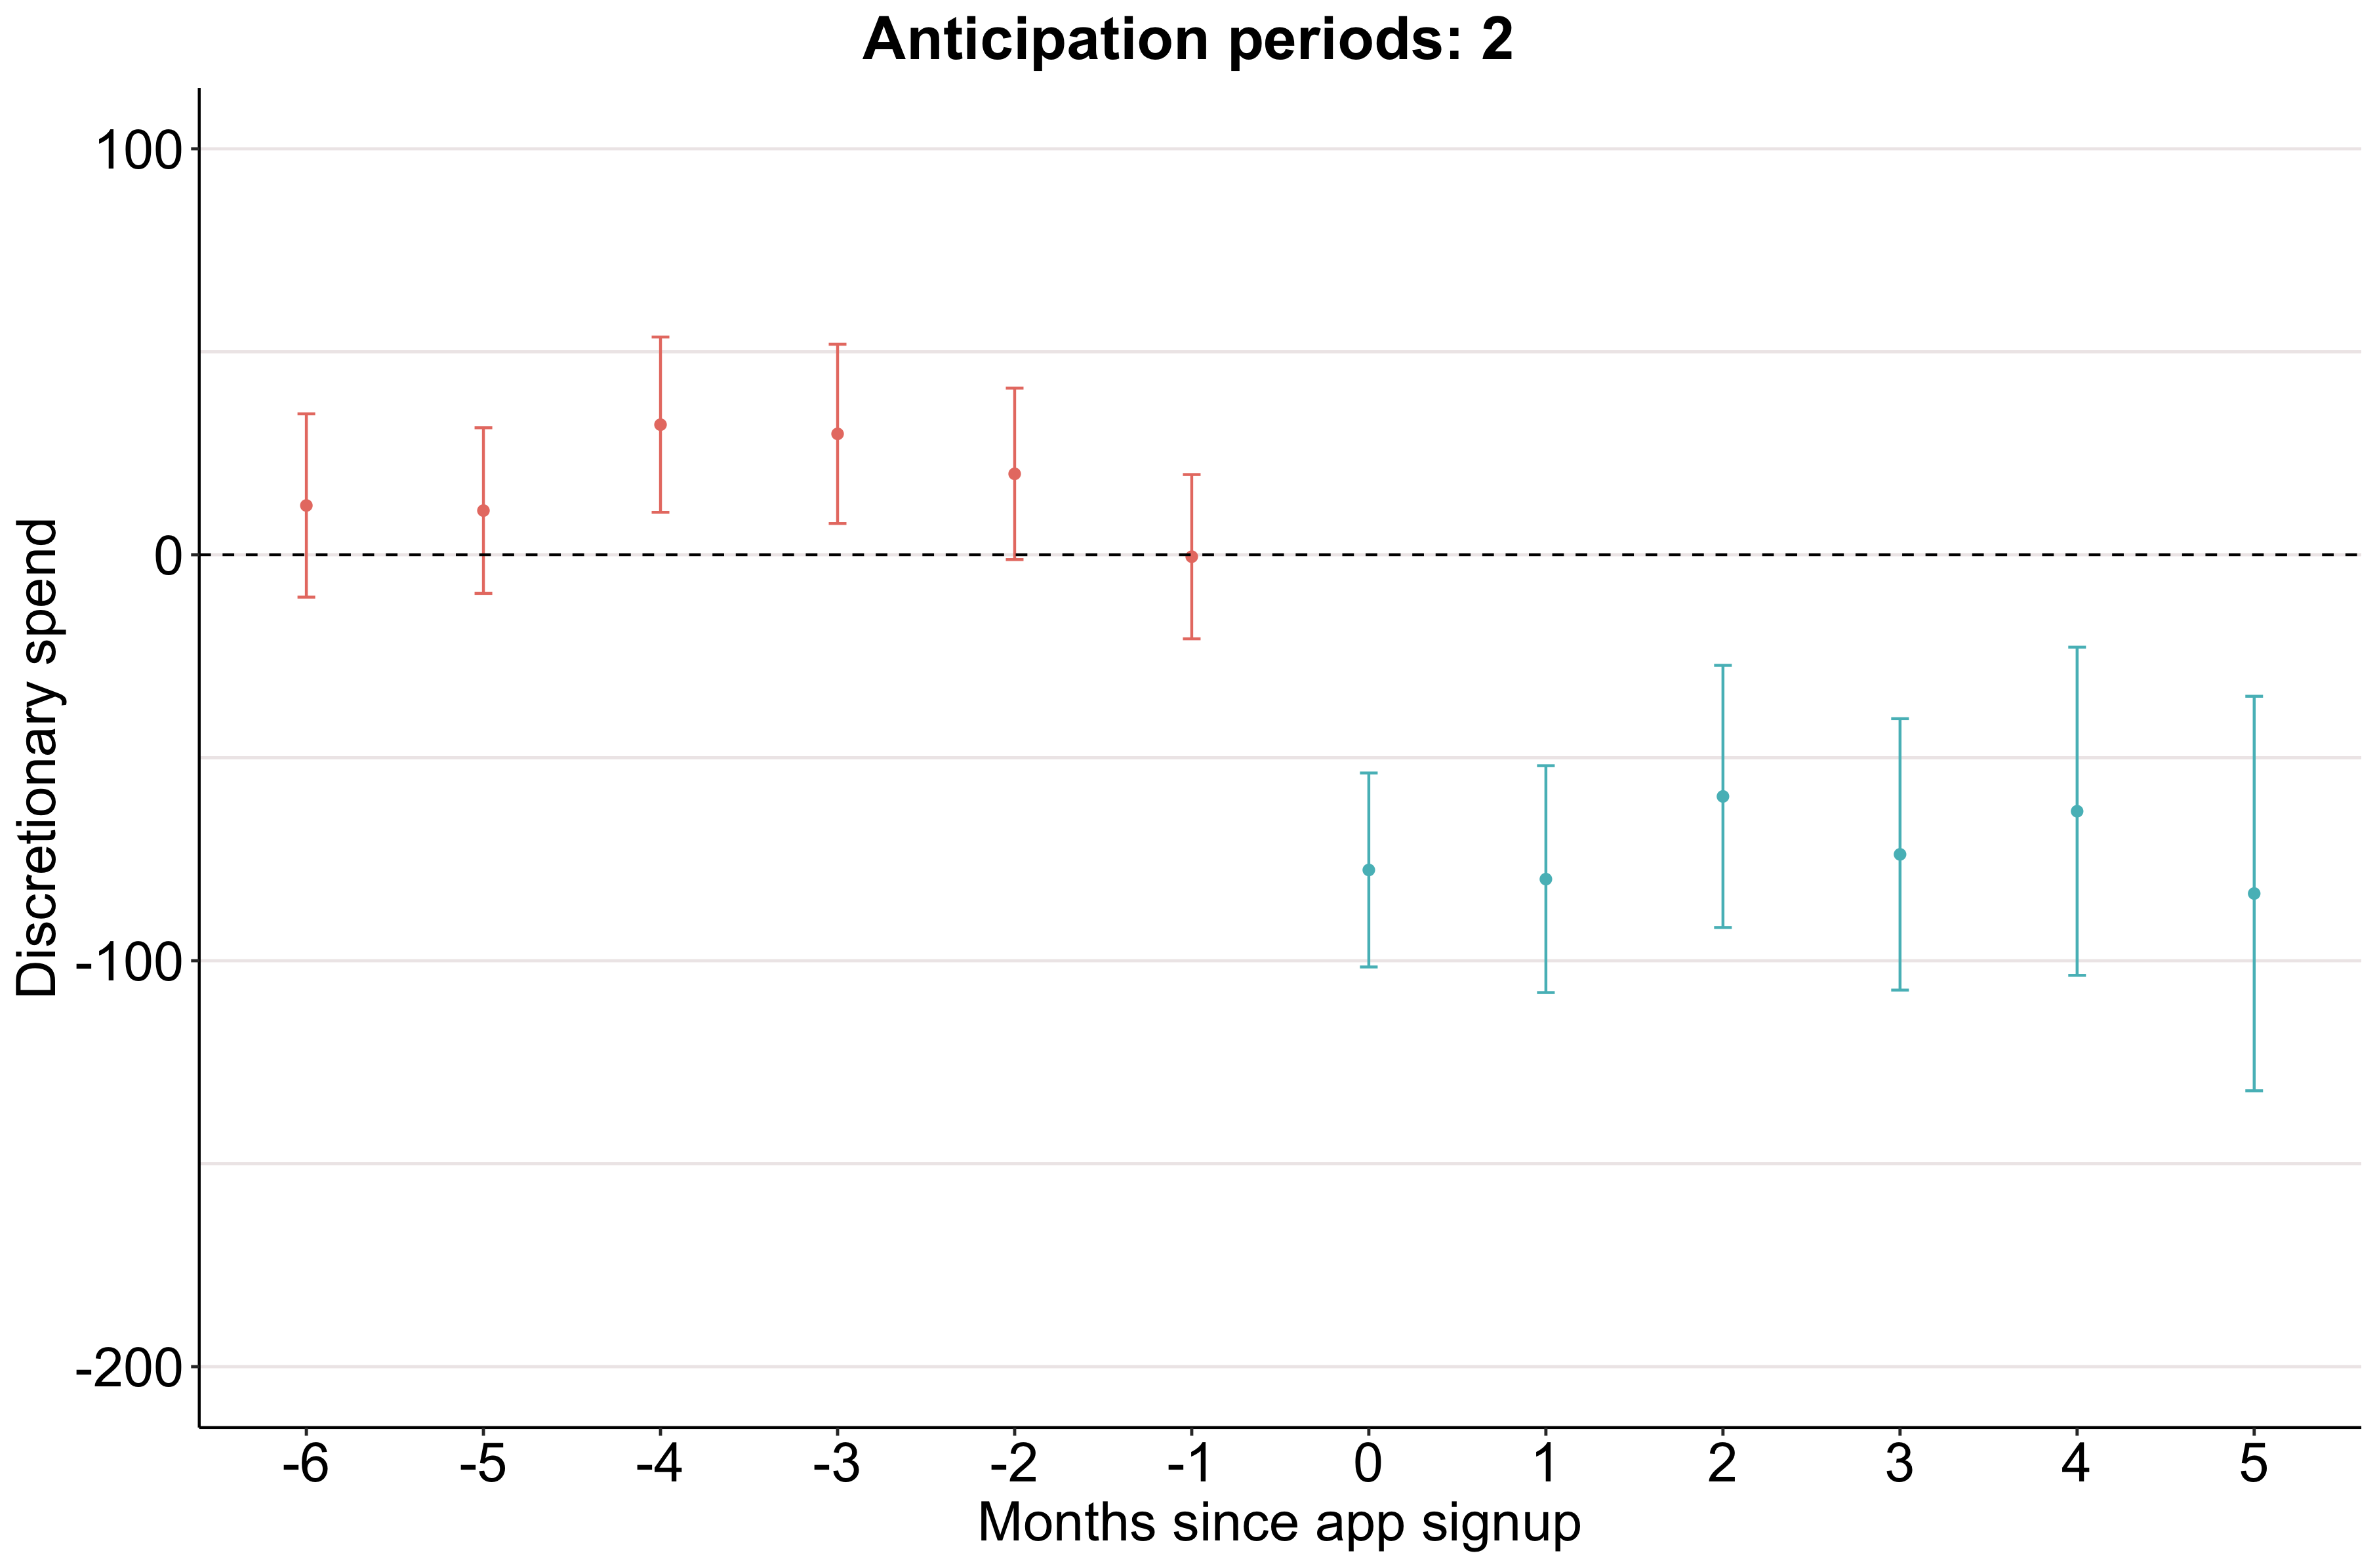
\includegraphics[width=.24\textwidth]{\figdir/dspend_antic2_es.png}
    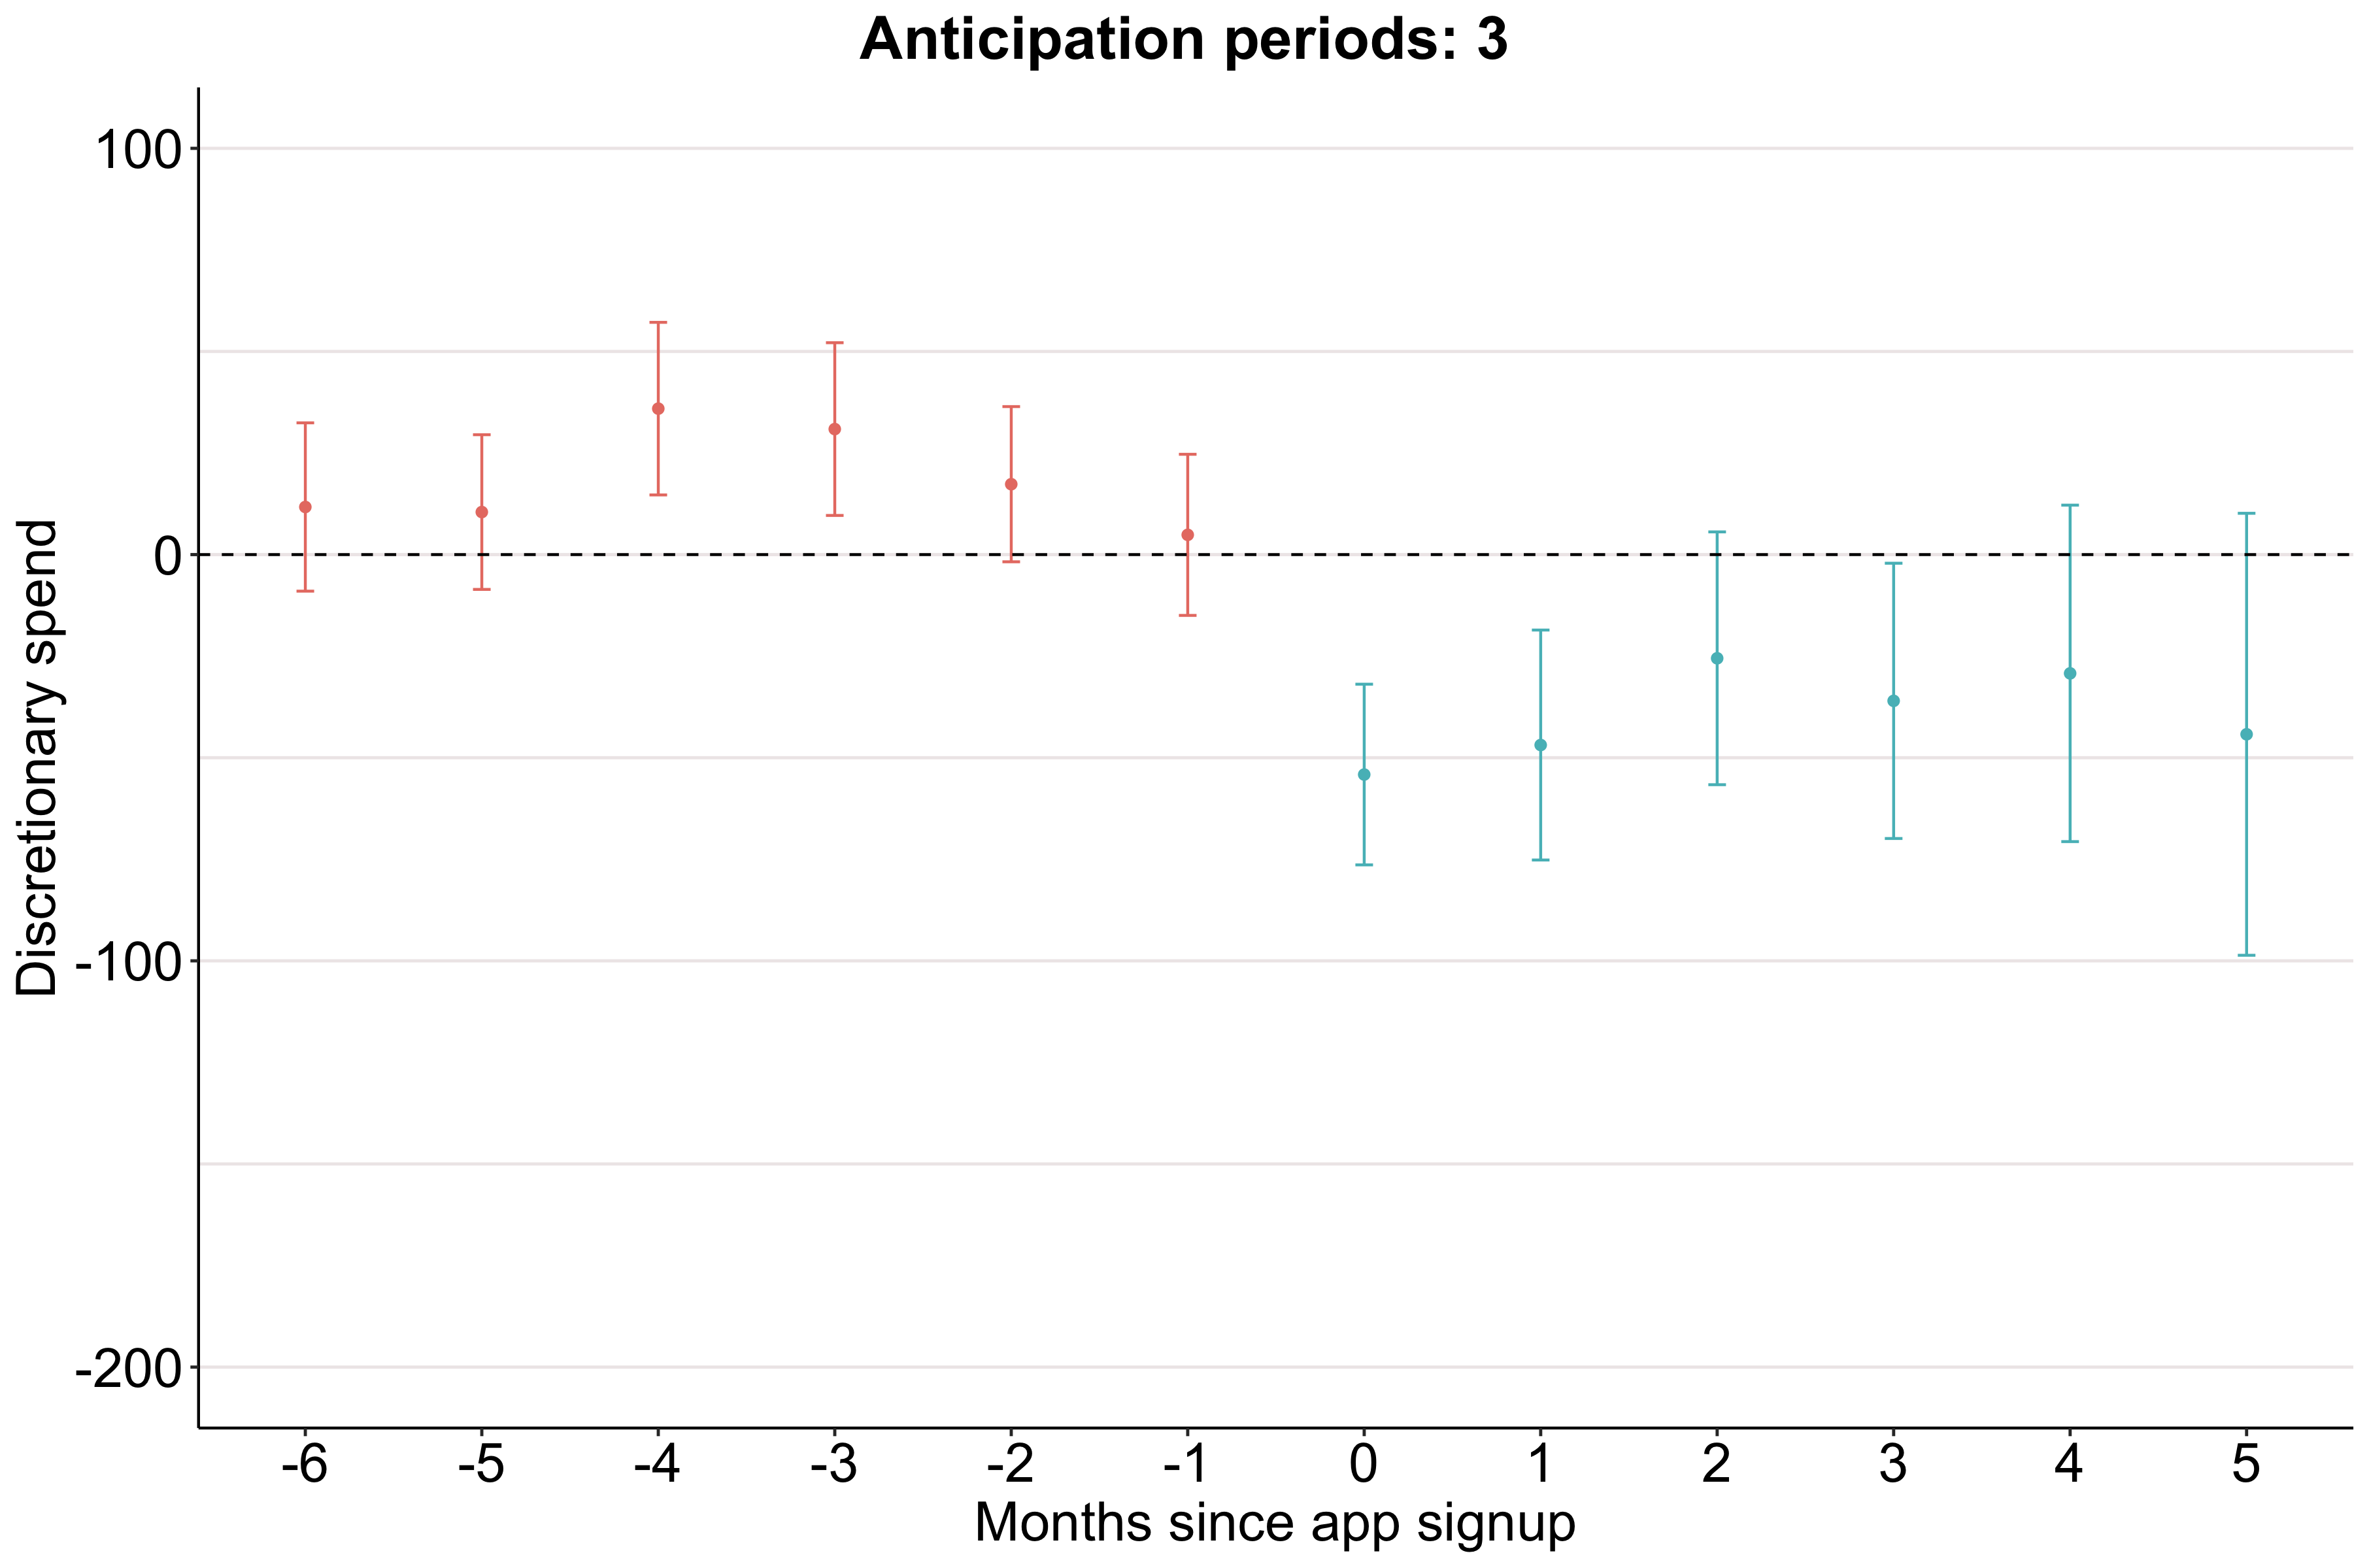
\includegraphics[width=.24\textwidth]{\figdir/dspend_antic3_es.png}
    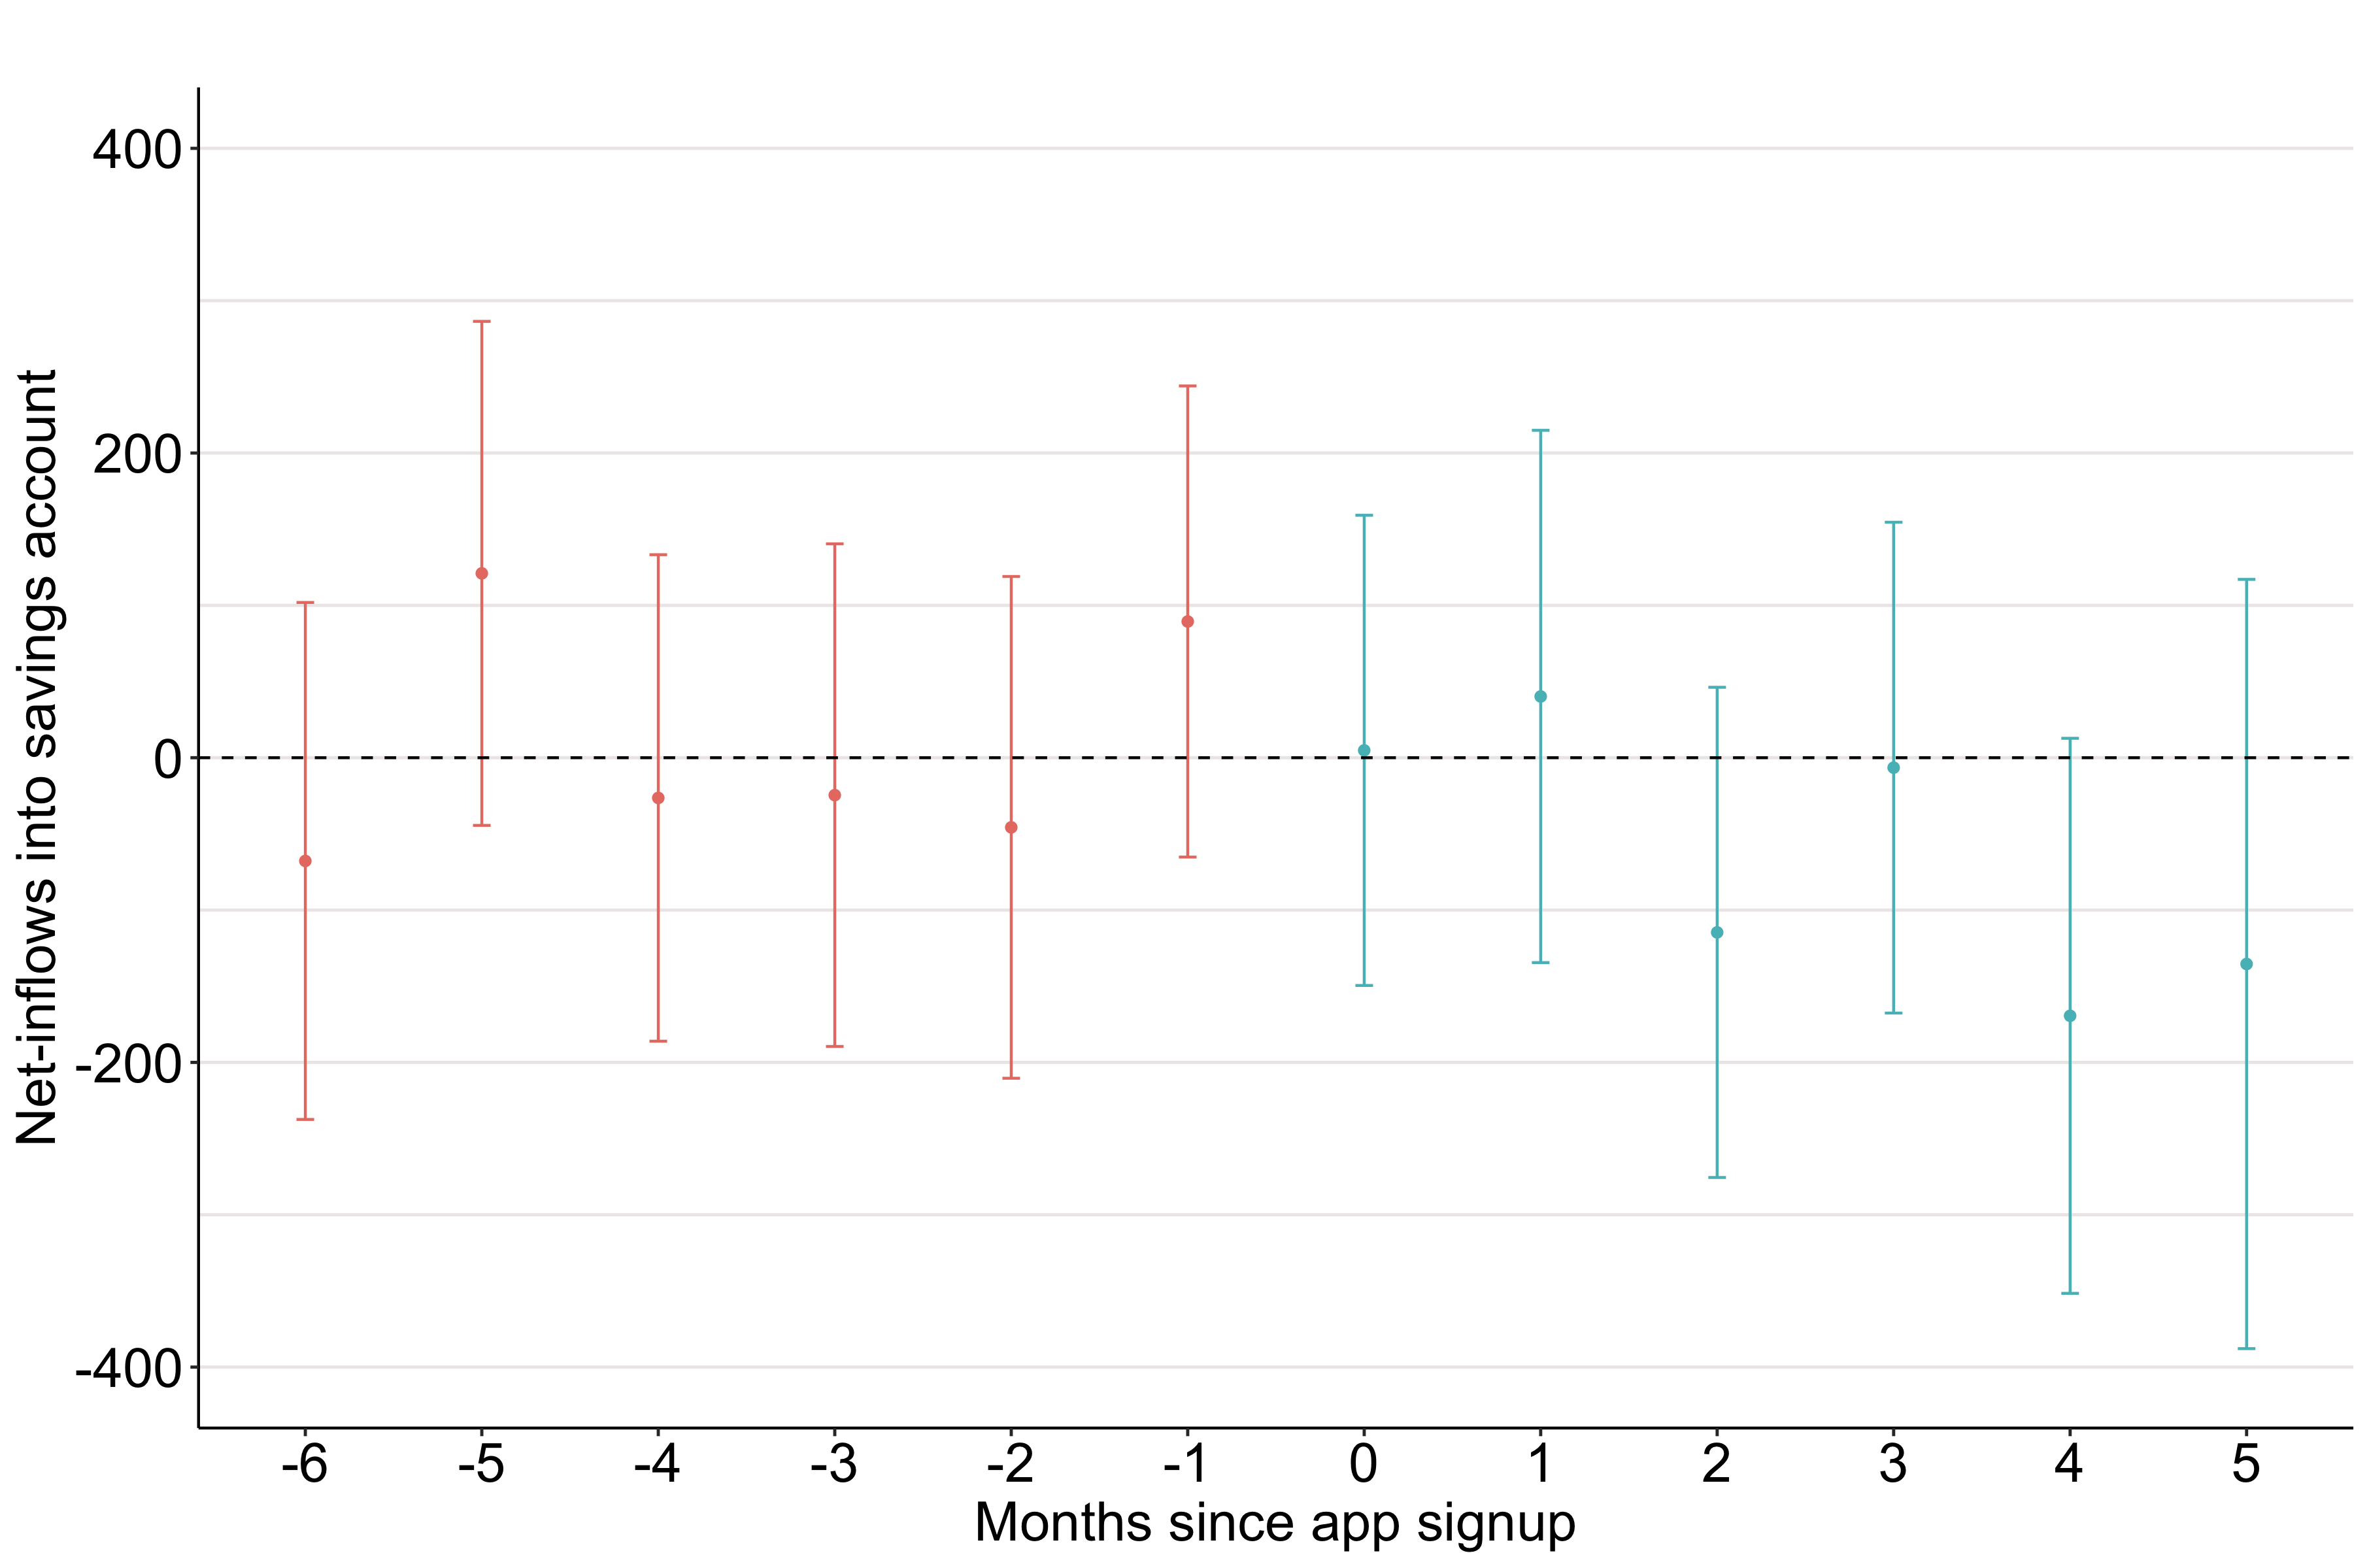
\includegraphics[width=.24\textwidth]{\figdir/netflows_antic0_es.png}
    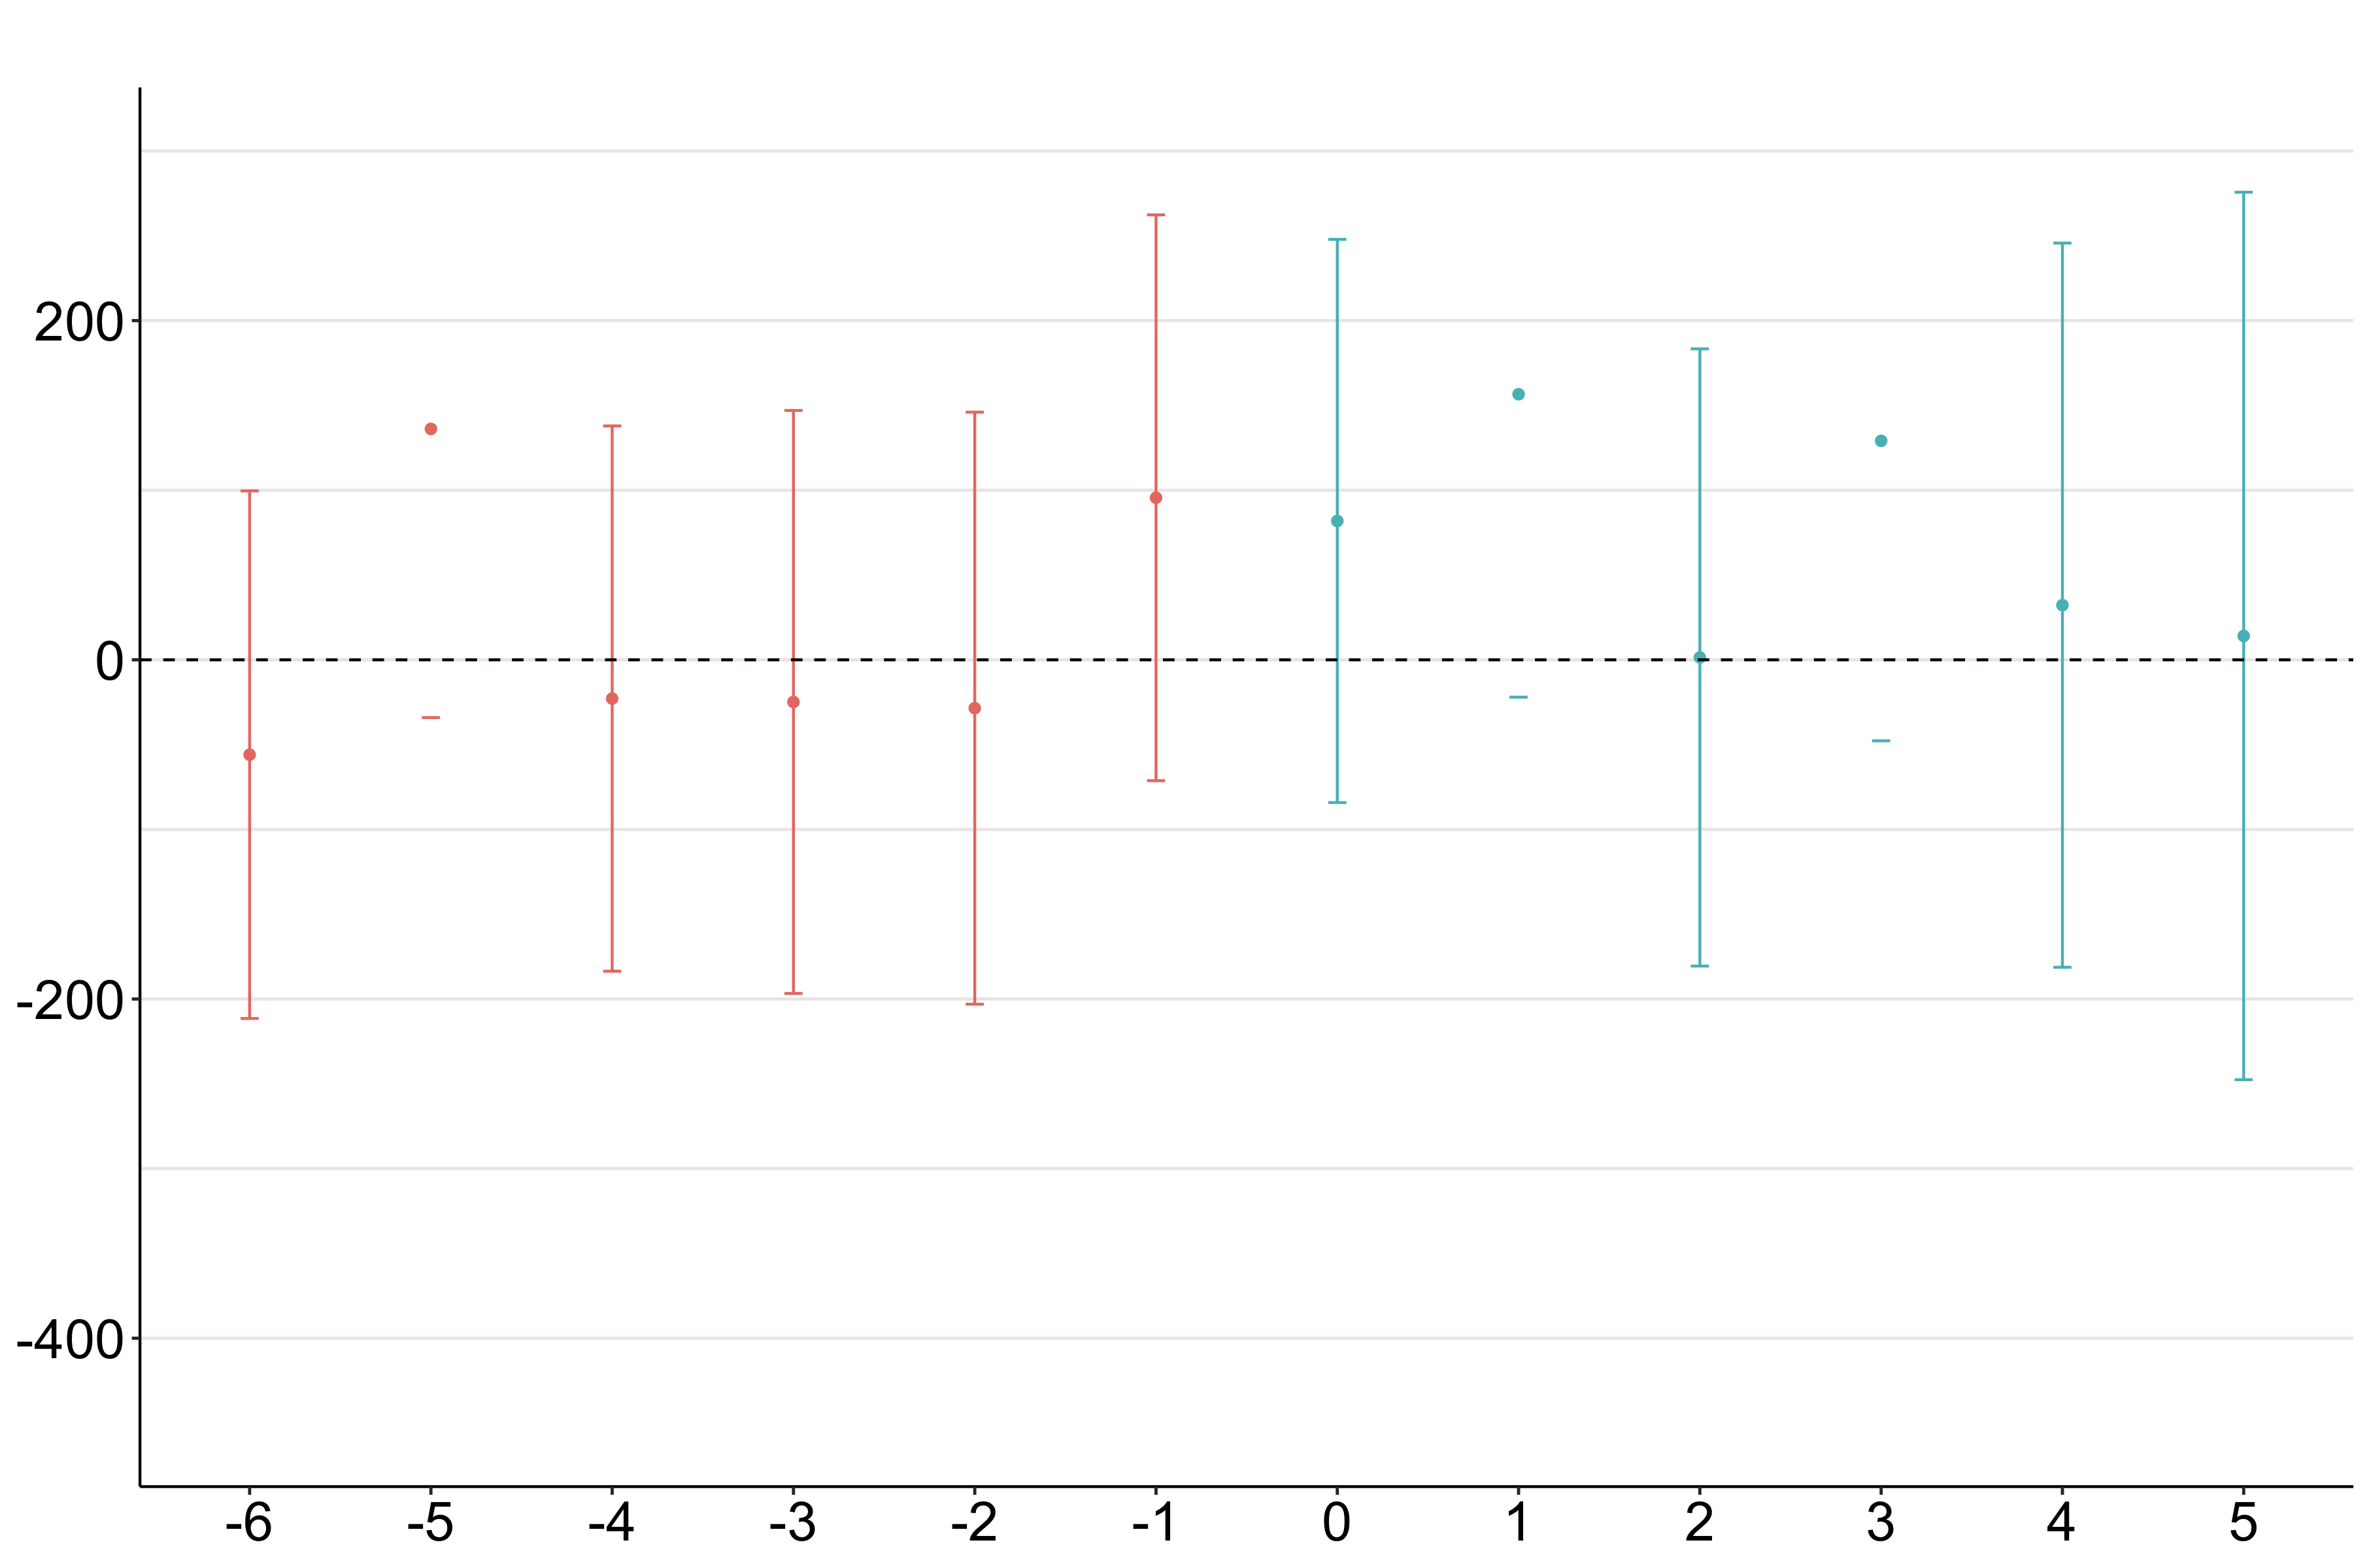
\includegraphics[width=.24\textwidth]{\figdir/netflows_antic1_es.png}
    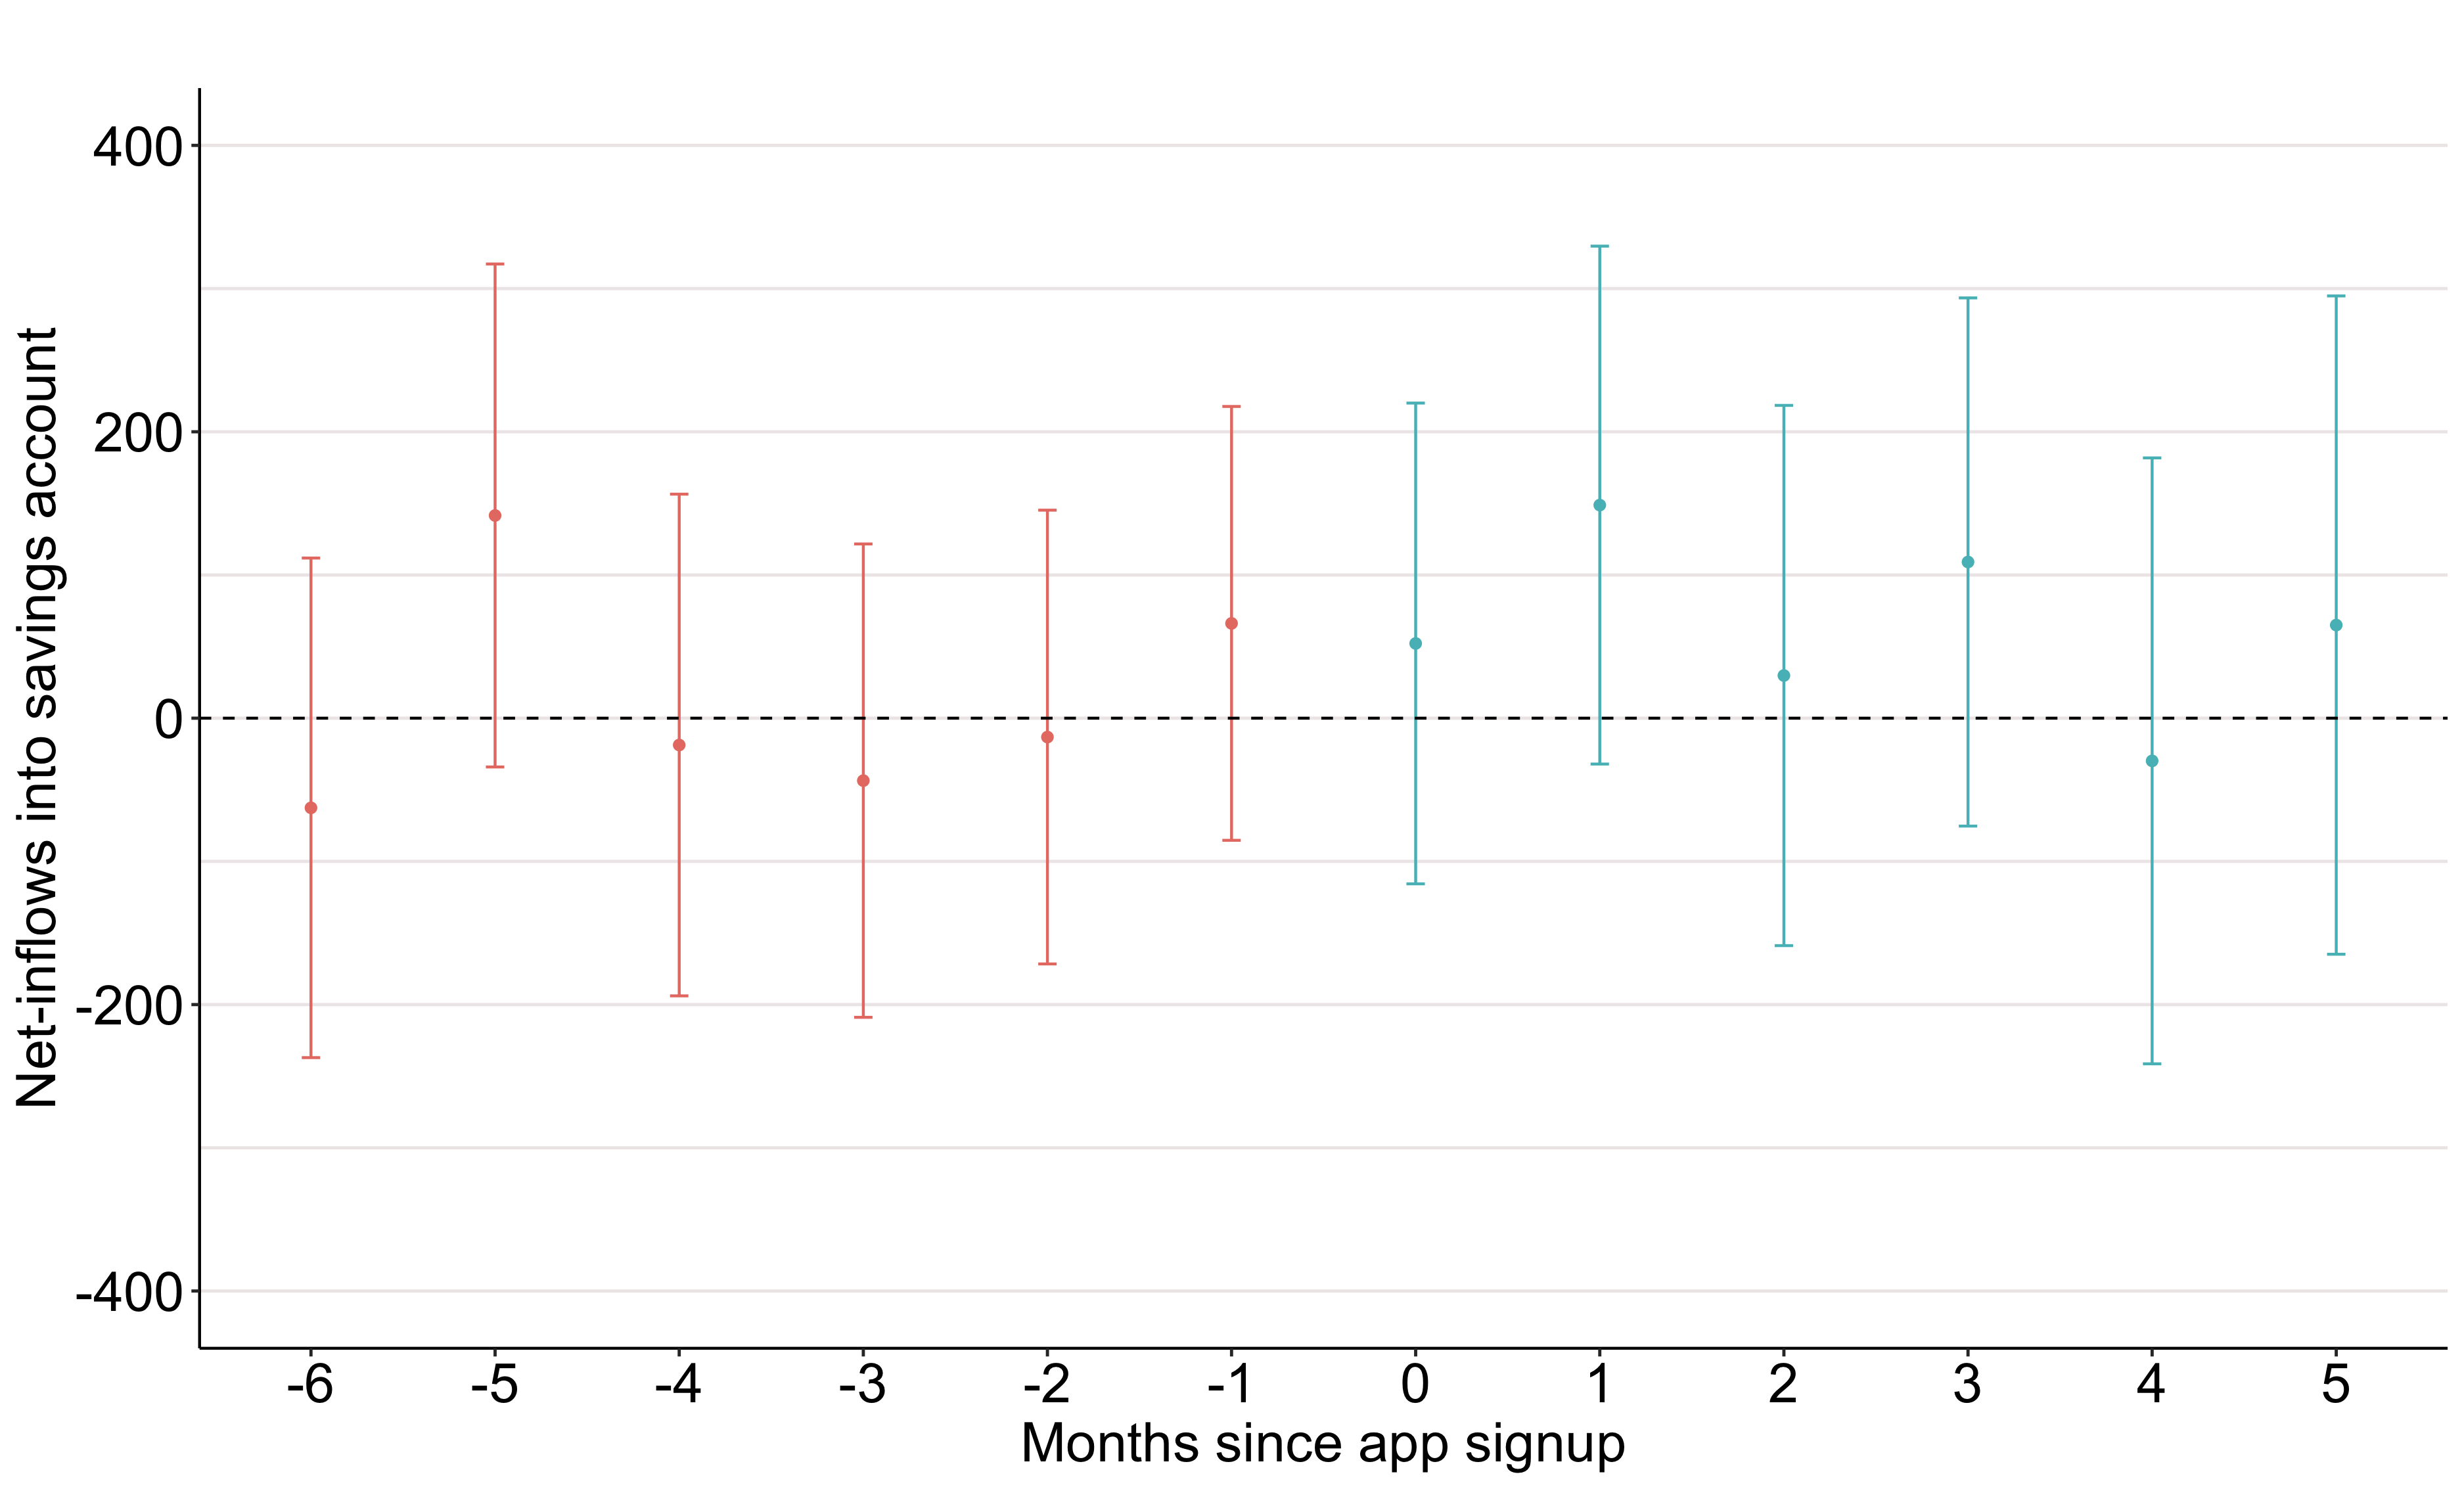
\includegraphics[width=.24\textwidth]{\figdir/netflows_antic2_es.png}
    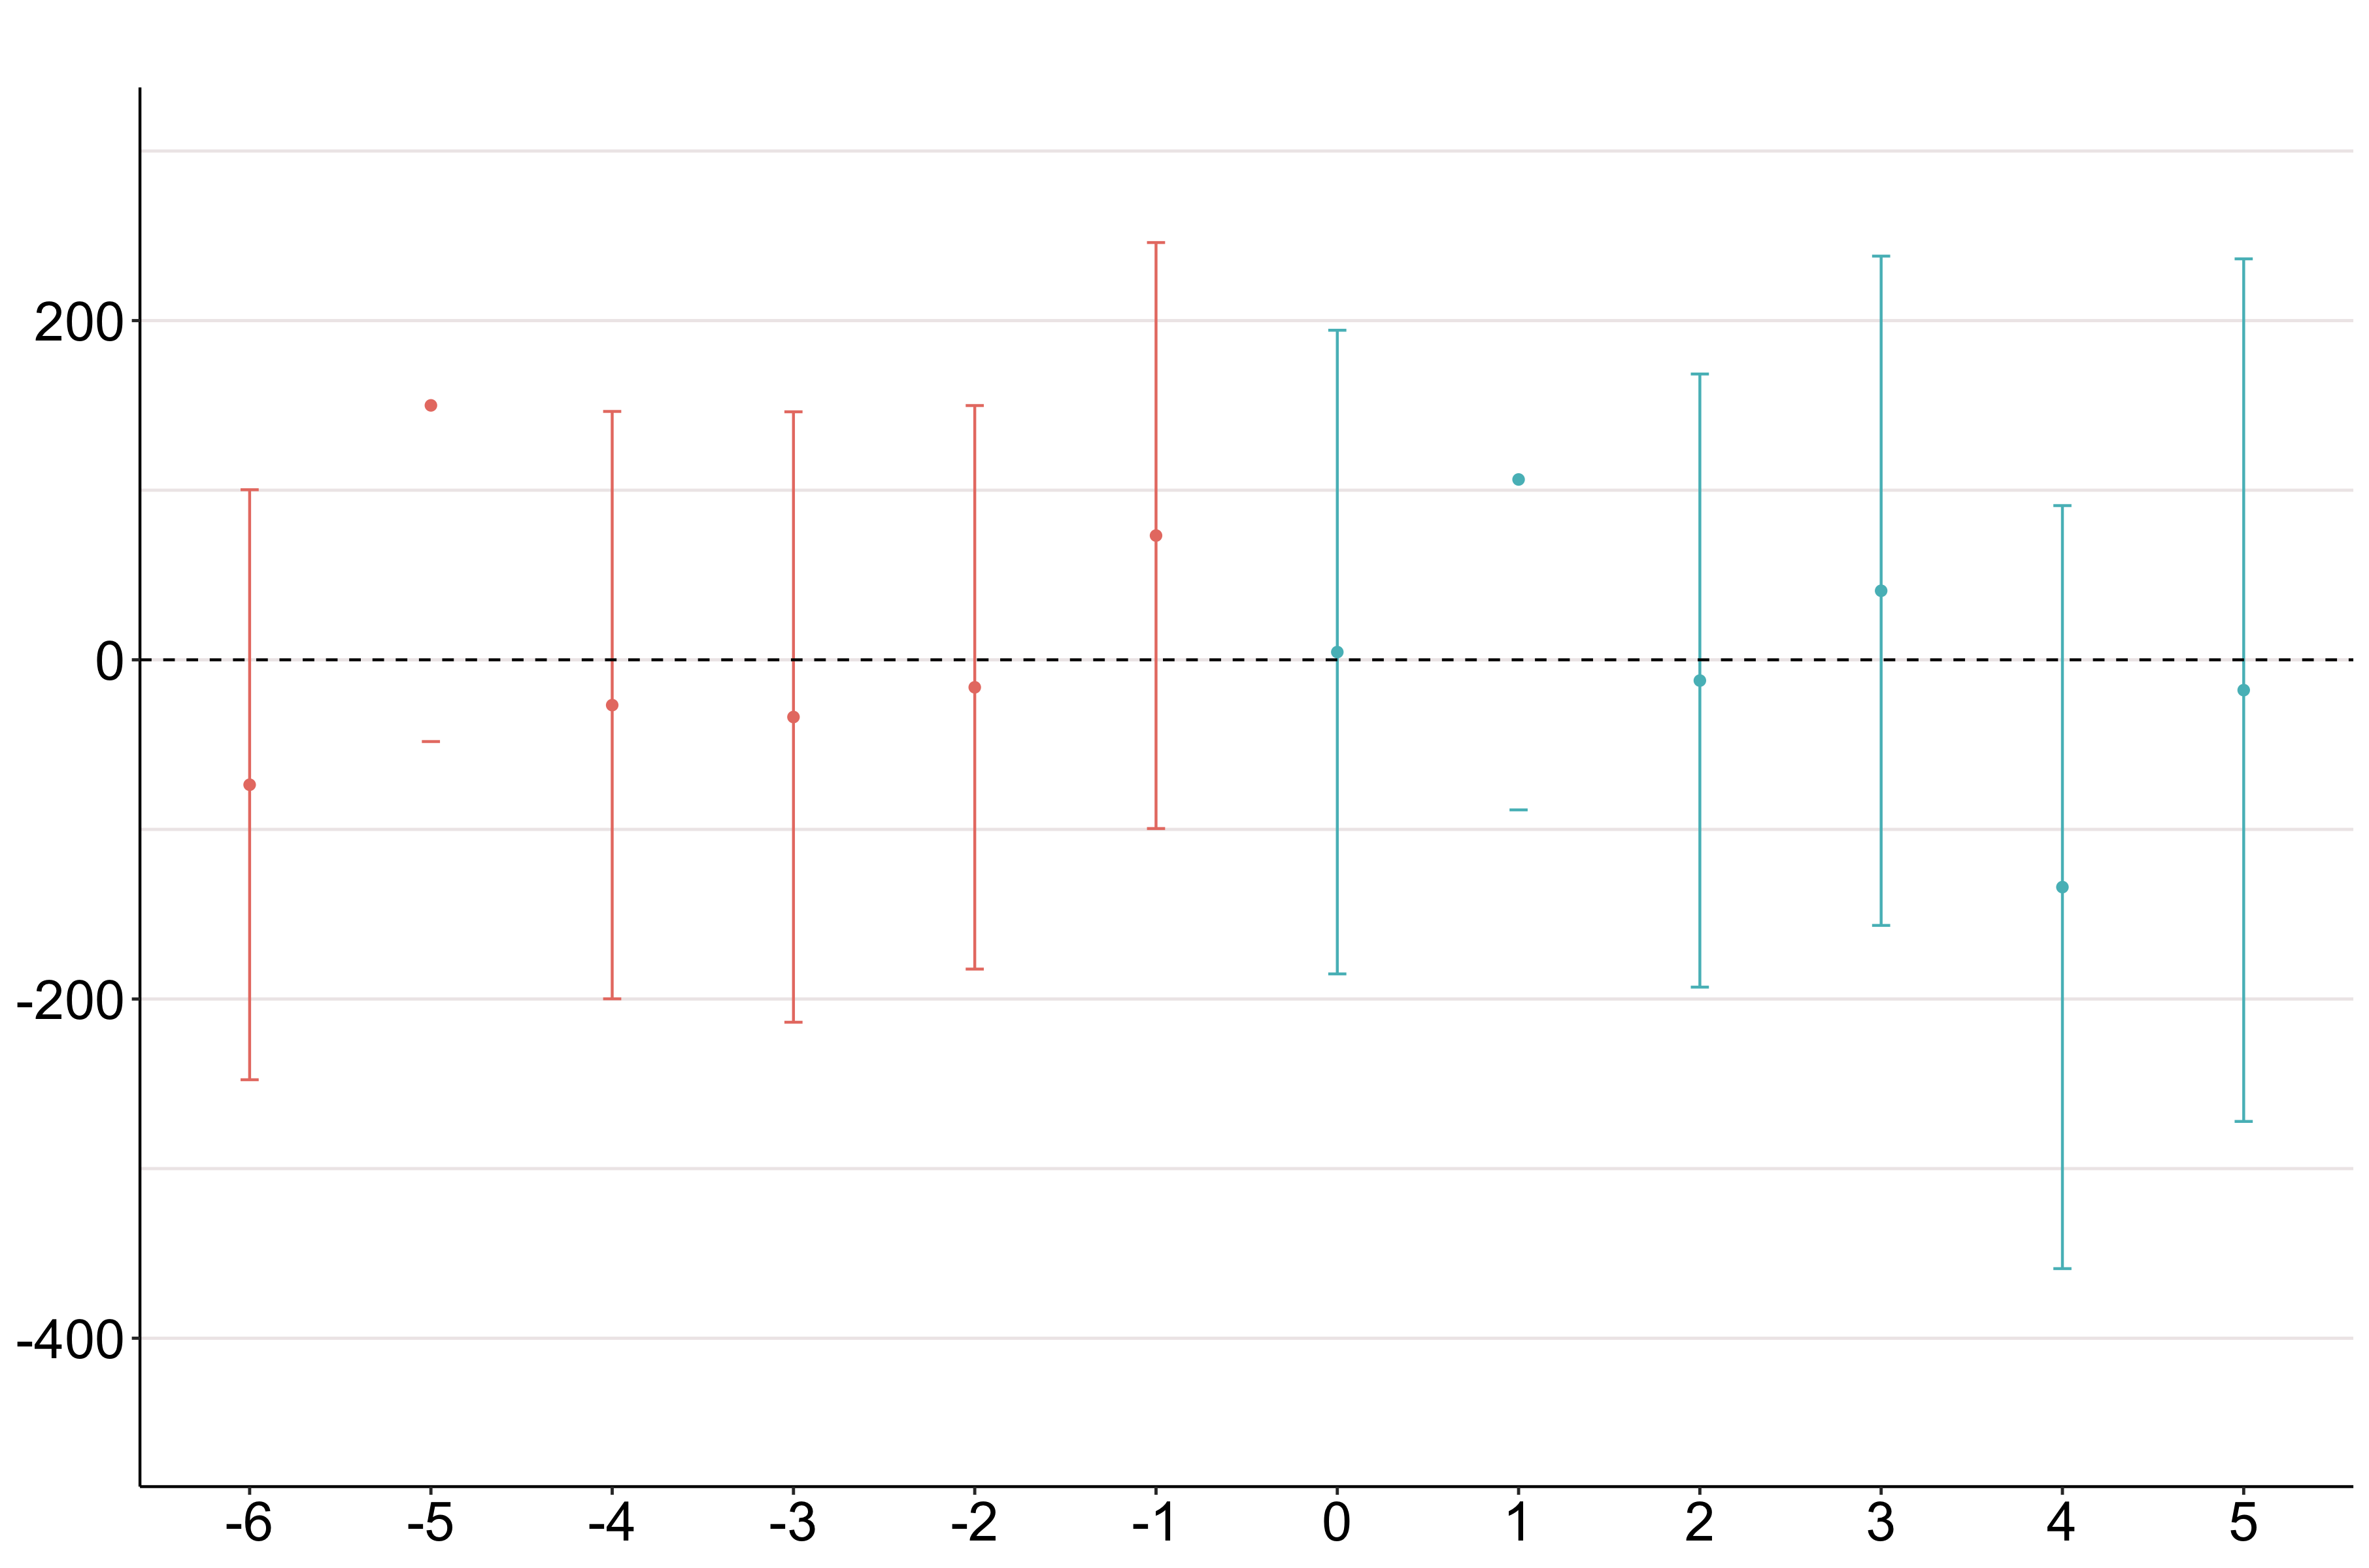
\includegraphics[width=.24\textwidth]{\figdir/netflows_antic3_es.png}
    \fignote{\textwidth}{...}
\end{figure}





